\documentclass[journal]{IEEEtran}

\ifCLASSINFOpdf
\else
\fi

%\hyphenation{op-tical net-works semi-conduc-tor}

\usepackage{graphicx}
\usepackage{epstopdf}
\usepackage{indentfirst}
\usepackage{cite}
\usepackage{verbatim}
\usepackage{amsmath}
\usepackage{multirow}
\usepackage{bm}
\usepackage{array}
\usepackage{subfigure}
\usepackage[colorlinks,
            linkcolor=red,
            anchorcolor=black,
            citecolor=green
            ]{hyperref}
            \makeatletter
\newcommand{\rmnum}[1]{\romannumeral #1}
\newcommand{\Rmnum}[1]{\expandafter\@slowromancap\romannumeral #1@}

 


\newcommand{\comments}[1]{}
\newcommand{\cxj}[1]{\textcolor{red}{(xuejin:#1)}}
\newcommand{\xjmd}[1]{\textcolor{blue}{#1}}
\newcommand{\vo}{\hat{\mathbf{v}}}
\newcommand{\vn}{\mathbf{v}}
\newcommand{\vset}{\mathbb{V}}




\makeatother
%\usepackage[justification=centering]{caption}
\begin{document}

\title{Efficient 3D City Modelling from Large-scale Aerial Images by Deep Learning}
%
%
% author names and IEEE memberships
% note positions of commas and nonbreaking spaces ( ~ ) LaTeX will not break
% a structure at a ~ so this keeps an author's name from being broken across
% two lines.
% use \thanks{} to gain access to the first footnote area
% a separate \thanks must be used for each paragraph as LaTeX2e's \thanks
% was not built to handle multiple paragraphs
%

\author{Feiyu Qin,
       Tongcun Zuo,
       Xuejin Chen}% <-this % stops a space
%\thanks{M. Shell was with the Department
%of Electrical and Computer Engineering, Georgia Institute of Technology, Atlanta,
%GA, 30332 USA e-mail: (see http://www.michaelshell.org/contact.html).}% <-this % stops a space
%\thanks{J. Doe and J. Doe are with Anonymous University.}% <-this % stops a space
%\thanks{Manuscript received April 19, 2005; revised August 26, 2015.}}

% The paper headers
%\markboth{Journal of \LaTeX\ Class Files,~Vol.~14, No.~8, August~2015}%
%{Shell \MakeLowercase{\textit{et al.}}: Bare Demo of IEEEtran.cls for IEEE Journals}
\maketitle

\begin{abstract}
Extracting buildings from remote sensing images plays an important role in urban applications (e.g., urban planning and digital city).
%
However, this task is quite difficult due to the great diversity of buildings and similarities between buildings and other categories.
%
Recent approaches have attempted to harness the capabilities of deep learning techniques for building extraction.
%
In this paper, we propose a robust method which extracts buildings from large-scale remote sensing images efficiently via deep learning. 
%
And further we extend our method to the 3D building reconstruction to accelerate the overall process.
%
Our study demonstrate that learning low-level appearance information and high-level semantic information are equally important in building extraction task since buildings possess various scales and aspect ratios in the scene.
%
Hence, to make full use of the information extracted from each layer, we propose a simple but effective hierarchical fusion operation which fuses the feature maps between channels stage by stage.
%
In this paper, a novel network named hierarchical fused fully convolution network(HF-FCN) is also described which fuses the information through combining the fusion operations to the general networks.
%
The experiments on several available remote sensing image datasets show that our method achieves state-of-the-art performance.
%
\cxj{Problem: Over-emphasized the buidling detection part, without clearly describe the scope of this paper and the relationship between detection and reconstruction. }
\end{abstract}
% Note that keywords are not normally used for peerreview papers.
\begin{IEEEkeywords}
building extraction, hierarchical fusion operation, Hierarchically Fused Fully Convolutional Network (HF-FCN), 3D city modelling
\end{IEEEkeywords}

%\IEEEpeerreviewmaketitle
%
\section{Introduction}
\label{sec:intro}


\cxj{Is your goal reconstruction or building extraction? The introduction should explain the overall goal. What are the challenges for building modeling from remote sensing images? What kind of work has been done in the literature? Why do we focus on building detection? What are our contributions?}

\IEEEPARstart{B}{uilding} extraction, which aims to extract rooftop\footnote{Because the data sets used in our article are high altitude remote sensing images which could be considered as the top views of the ground. Therefore, we do not distinguish the concepts of buildings and rooftops in the subsequent description.} in a large-scale remote sensing image, remains one of the main challenges have been studied for decades in the field of remote sensing. Moreover, automatic extraction of building rooftops from aerial and satellite imagery is an important step in many applications, such as: urban planing, automated map making, 3D city modeling, updating geographical dataset and military reconnaissance. It is particularly difficult to extract rooftop from remote sensing images at the pixel level because of the following three reasons: \romannumeral1) Density of the structures in the scene. A rural scene has low density but an urban scene has high density, with a suburban scene in between (medium density).  \romannumeral2) Shape of the structure. Buildings come in many shapes from simple rectangular blocks with flat roof to complex shapes with intricate, multi-based roof structure.  \romannumeral3) Image quality. Images vary in terms of contrast, resolution, and visibility  \cite{IEEEexample:huertas1988detecting}. Some remote sensing patches are shown in Fig.~\ref{fig:intro} \cxj{do not use the figure no directly. using ref{}..} , which illustrate the challenges of building extraction task.


\begin{figure}
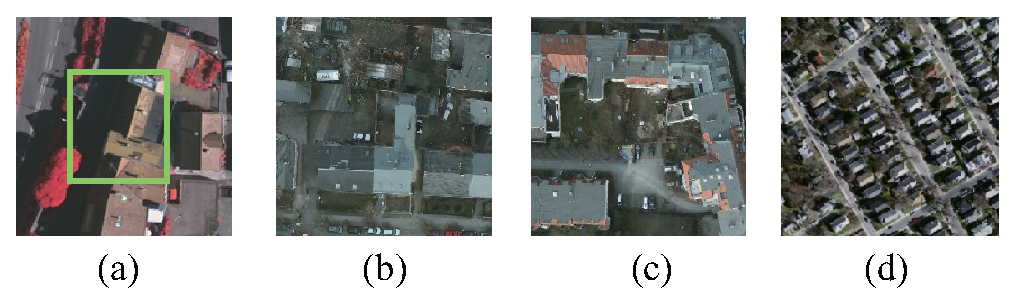
\includegraphics[width=8.7cm]{Figures/challenge.eps}
\caption{Examples of remote sensing patches with different kinds of challenges. (a) Shadow occlusion in green frame. (b) Low inter-class differences. (c) High intra class variance. (d) A lot of tiny buildings close to each other.}
\label{fig:intro}
\end{figure}


In the past decades, many researchers made some experimental investigations to extract buildings automatically. In the early days, many knowledge-based methods were put forward by \cite{IEEEexample:huertas1988detecting}, \cite{IEEEexample:noronha2001detection}, \cite{IEEEexample:nosrati2009novel}, \cite{IEEEexample:izadi2012three}, \cite{IEEEexample:wang2015efficient} whose basic ideas are derived from prior knowledge of buildings, for instance, buildings are closed polygons made up of some straight lines. Some others are energy based methods which mainly includes the variational level set evolution, improved snake model and graph cut \cite{IEEEexample:cote2013automatic}, \cite{IEEEexample:peng2005improved}, \cite{IEEEexample:sirmacek2009urban}.


In recent years, with the development of machine learning, many machine-learning techniques are gradually penetrating into the remote sensing domain.
At first, some shallow networks were proposed for multiple object extraction\cite{IEEEexample:mnih2013machine}, \cite{IEEEexample:saito2016multiple}, \cite{IEEEexample:alshehhi2017simultaneous},\cite{IEEEexample:zhao2017contextually}. Afterwards, with increasing computer power, deep learning developed rapidly and introduced into the field of remote sensing. At the same time, some researchers tried Convolutional Neural Networks (CNNs) for aerial images classification and semantic pixel labelling~\cite{IEEEexample:paisitkriangkrai2015effective}, \cite{IEEEexample:liu2017dense}, \cite{IEEEexample:audebert2017deep}, \cite{IEEEexample:kampffmeyer2017urban}, \cite{IEEEexample:he2017multi}.


In this work, a relatively simple, but very effective, manner is proposed and combined into a general CNN architecture for building extraction. We take full advantages of the low-level appearance information as well as high-level semantic information by the novel fusion operation in a way of stage by stage.
Numerous experiments conducted on three remote sensing image datasets all obtain fairly good results.
We further extend our work to the field of 3D modeling as the part of building detection. And it be easily intergrated into the pipeline of building reconstruction.
Our technical contributions are:
%
\begin{enumerate}
	\item A effective hierarchical fusion operation which is specially designed for multi-scale building extraction is proposed. Combining with a trimmed VGG16 Net, a novel network is presented, named HF-FCN that can deal with the problems of different sizes, diverse appearance and mutual occlusion of buildings and etc.
	\item HF-FCN is an end-to-end network that does not need any post processing. And the approach is significantly computationally efficient than existing techniques. Besides, the overall accuracy based on HF-FCN exceeds the state-of-art algorithms.
	\item A extend exploration for building reconstruction of large-scale urban areas is studied. And the experiments reveal the method well preserve buildings details.
\end{enumerate}

The remainder of this paper is organized as follows. Sec.~\ref{Sec:RelatedWork} sums up the related works in the past.
In Sec.~\ref{Sec:HF-FCN}, we introduce the fusion operation and architecture of HF-FCN. The training steps are also presented.
And in Sec.~\ref{Sec:exp}, a brief description of the dataset used for our task is provided. HF-FCN training strategies, details and its evaluation metrics are also described.
In Sec.~\ref{Sec:Res},we display and analysis the experimental results.
Extension in 3D building modeling are presented in Sec.~\ref{sec:app}.
Finally, the conclusion is discussed in Sec.~\ref{Sec:Con}.

\section{Related Work}
\label{Sec:RelatedWork}
Building extraction is one of the most fundamental problems in remote sensing domain, which has been studied for nearly 30 years. Meanwhile, many research achievements have sprung up. As time goes by, we can roughly divide these methods into three groups: one is based on the shape prior, another is based on the energy function and machine learning third. Here we briefly review some representative methods that have evolved in the past decades.\par
\setlength{\parindent}{2ex}During early days, methods are mainly based on the hypothesis of prior knowledge. Huertas et al \cite{IEEEexample:huertas1988detecting} assumed that buildings are rectangular or composed of rectangular components. Based on this, the approach detected lines and corners, traced object boundaries and used shadows to verify. Later, a system \cite{IEEEexample:noronha2001detection} for building detection and modelling was proposed with the assumption that the roofs were flat or symmetrical and walls were vertical. Using known ground height and detected rooftop, the reconstructed models could be soon obtained. Further, Nosrati \cite{IEEEexample:nosrati2009novel} transformed the line and intersection points of the image into a graph presentation, and turned the problem of polygon finding into the one that finding loops in the graph. However, it was still estimated on assumption that the buildings are polygonal. In addition, Izadi \cite{IEEEexample:izadi2012three} presented a complete system for building detection and modelling. In the stage of building detection, a tree consisting of intersection points of lines was created and refined based on the found hypotheses. The sun azimuth and elevation angles were used to estimate the height with existing shadows afterwards. As the height of buildings estimated, the three-dimensional polygonal building models were built. In recent years, very high resolution (VHR) optical satellite imagery could be obtained easily. Hence, Wang \cite{IEEEexample:wang2015efficient} proposed an efficient method for automatic rectangular building extraction from VHR remote sensing images by detecting line segments and grouping lines based on path integrity and closed contour search.\par
\setlength{\parindent}{2ex}The aforementioned shape-based methods seem to have a good performance in rural scenes with low density of buildings. Neverthless, there are some limitations of these methods. First, the shape-based methods inherently limited to handle buildings of arbitrary shapes. Second, these methods may failed to deal with complicated cases, for instance, buildings are close to each other, which thereby is hard to adapt to today's applications. Third, the method using shadows to verify corners and estimate height is greatly limited to obvious shadows and sparse building environment. \par
\setlength{\parindent}{2ex}Later, several energy-based methods have been applied in automatic rooftop extraction. Cote \cite{IEEEexample:cote2013automatic} employed corner detection as an initial estimate of the roof, and then refined with level set evolution. Peng and Liu \cite{IEEEexample:peng2005improved} proposed an approach that segments remote sensing images into high objects, ground and shadow regions, with further refined by an improved snake model. The urban-region-detection problems were casted as one of multiple subgraph matching by Sirmacek et al \cite{IEEEexample:sirmacek2009urban}. They considered each SIFT keypoint as a vertex, neighborhood between vertexs as edge of the graph and formulated the problem of building detection in terms of graph cut.\par
\setlength{\parindent}{2ex}Over the past decade, CNNs have achieved great success in the field of computer vision. There are significant amount of efforts on semantic pixel-level classification for extraction buildings in remote sensing. A shallow patch-based network was proposed by Mnih \cite{IEEEexample:mnih2013machine} which has only five layers with a 64 by 64 aerial patch as input. And the output of the network was processed by conditional random fields (CRFs). Afterwards, Satio et al.\cite{IEEEexample:saito2016multiple} applied two major strategies to improve the performance of the network. One was a channel-wise inhibited softmax (CIS) for getting a multi-label prediction result, the other was model averaging with spatial displacement (MA) for enhancing the prediction result. Alshehhi et al. \cite{IEEEexample:alshehhi2017simultaneous} also adjusted the architecture of network proposed by Mnih through changing the kernel size of convolutional layers and replacing the fully connection layer of the last layer with the average pooling layer. Alternative post-processing strategies such as CRFs and multi-scales were used to improve the final prediction results. Some methods took advantage of the feature extraction capability of CNNs to generate feature descriptions of patches. Paisitkriangkrai et al. \cite{IEEEexample:paisitkriangkrai2015effective} made use of both the CNN and hand-craft extracted features, which were combined together to generate predicted labels of each patch. They also used CRFs as post-processing to get a sound result. Zhao et al. \cite{IEEEexample:zhao2017contextually} proposed a method using edge information of VHR to guide semantic segmentation. Unlike \cite{IEEEexample:paisitkriangkrai2015effective}, \cite{IEEEexample:he2017multi} put forward a multi-label pixelwise classification method using the feature vector extracted by a CNN to train a Support Vector Machine (SVM) for classification.\par
\setlength{\parindent}{2ex}More recently, Long \cite{IEEEexample:Long_2015_CVPR} illustrated that Fully Convolutional Networks (FCN) could better handle the problem of multi-label pixel-wise classification. By up-sampling, final predicted result could be the same resolution of the input. Liu et al. \cite{IEEEexample:liu2017dense} did a further research on the formulation proposed by Paisitkriangkrai \cite{IEEEexample:paisitkriangkrai2015effective} but used FCN as the branch of CNN and applied a higher-order CRFs as post-processing. Unlike traditional CRFs, the label consistency for the pixels within the same segment were enforced by higher-order CRFs. In order to reduce the information loss during pooling stage, SegNet \cite{IEEEexample:badrinarayanan2017segnet} delivered pooling indices computed in the max-pooling to the decoder. It eliminated the need of learning during the up-sample stage while achieving good segmentation performance. The SegNet architecture was used by Audebert et al. \cite{IEEEexample:audebert2017deep} for semantic labeling of remote sensing and got better prediction results compared to the traditional methods. Later, Kampffmeyer at al. \cite{IEEEexample:kampffmeyer2017urban} proposed a novel idea that using CNN with missing data for urban land cover classification. The idea came from a modality hallucination architecture proposed by Hoffman et al. \cite{IEEEexample:hoffman2016learning} which learned with side information during training stage.\par

Although above-mentioned CNN-based models have exceeded the traditional methods significantly, all of them lost important hierarchical features extracted from shallow layers. They usually apply the CNN features from the last layer to get a segmentation result. It may omit tiny objects during the process of pooling, and could not handle the situation when the size of buildings have great difference in distribution. Aiming at this case, a hierarchically fused fully convolutional network is proposed to combine features extracted from each convolutional layer to capture detailed information of input. We will show the details of our idea below.

\section{Hierarchically Fused Fully Convolutional Network}
\label{Sec:HF-FCN}
In this section, we introduce a novel operation for feature fusion, named hierarchical fusion operation and apply it to the common networks, VGG16 Net and ResNet. The overview diagram in Fig.~\ref{fig:Fusion-Operation} shows where the fusion operations take effect and how they work. Different from other networks for semantic segmentation, we apply the fusion operation twice to integrate information gradually.
Our network consists of three parts. Part 1 is a bottom-up pathway which plays a role of features extractors at different levels.
In theory, arbitrary feature extraction network is applicable to the Part 1.
The second part is a process of feature fusion in the first stage, which fuses the feature maps generated from Part 1.
Besides, Part 3 is a second stage of feature fusion.
In Part 3, we take full advantage of the information extracted from the Part 2 by learning the connection weights between upsampled feature maps.

\begin{figure}
\centering
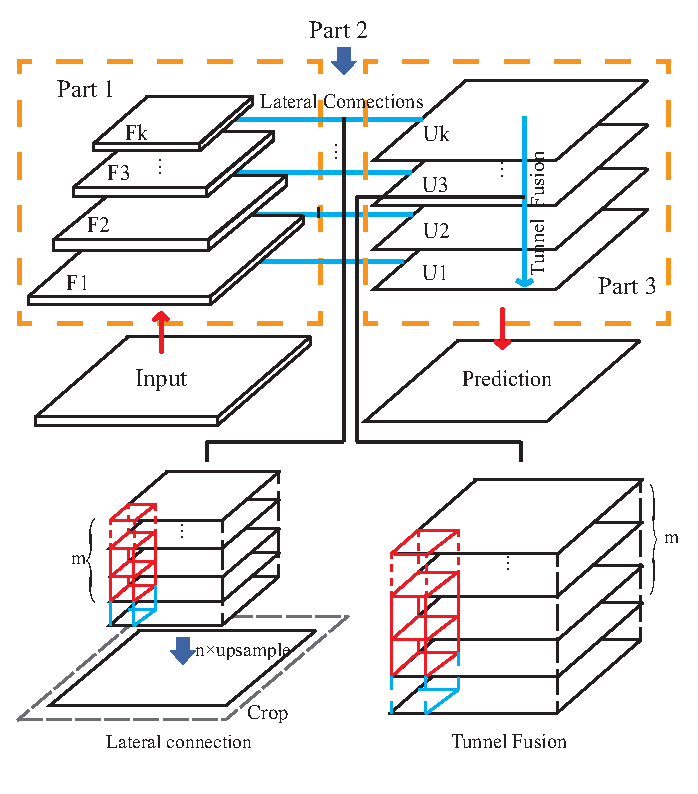
\includegraphics[width=8.5cm]{Figures/Fusion_Operation.eps}
\caption{The first line shows the overview of our network. The second row shows the details of two kinds of fusion operation. One is a case where the input is not equal to the output and the other is the input equal to the output. Fk means the feature maps come from the kth layer. m for number of feature maps. n said the n times of up sampling.}
\label{fig:Fusion-Operation}
\end{figure}
\cxj{Put overview here. Explain the main components of our methods.}
\subsection{Network Architecture}

\textbf{Part 1} The Part 1 is a bottom-up pathway, which generates the hierarchical feature maps from the network. With the increase of the field of perception, the extracted semantic information is gradually from the lower level to the high level. At the same time, the extracted information of image is from local to global. Each group of feature maps come from the same convolution(conv) layer contribute to the ${\left\{F_{k}\right\}}$ in Fig.~\ref{fig:Fusion-Operation}, where ${k:\Omega \to\left\{1,\ldots,K\right\}}$. And ${K}$ is the number of groups; for instance, ${K}$ is 13 for VGG16 Net. Specifically, for ResNets, we consider a ResBlock as a feature extractor that ${K}$ is 15.

\textbf{Part 2} The Part 2 which fuses the feature maps of each group extracted from Part 1 via a set of hierarchical fusion operations. Due to the feature maps learned from same group including similar types of information, we fuse them into one feature map, which contains the richer features. The hierarchical fusion operation consists of three steps:
A ${1\times1}$ conv layer first, deconvolutional (transposed convolution) layer second and crop operation third. 
The Part 2 in Fig.~\ref{fig:Fusion-Operation} can be written as:
\begin{equation}
    \label{fusion_1}
    \ U_{k}=Crop(UpSample_n(Conv(\left\{F_{k}\right\})))
\end{equation}

where ${\left\{F_{k}\right\}}$ is extracted feature maps from Part 1, ${k:\Omega \to\left\{1,\ldots,K\right\}}$. 

The first step is a ${1\times1}$ conv operation among the channels of feature maps in the same group.
${Y = Conv(\left\{X\right\})}$ is defined as:
\begin{equation}
    \label{Conv}
    \ Y(i,j)=\sum_{m=1}^{M}w_{m}X_{m}(i,j)
\end{equation}

 where ${M}$ is the number of the feature maps in ${\left\{X\right\}}$. The ${w_{m}}$ is the weight of conv kernels, ${m:\Omega \to\left\{1,\ldots,M\right\}}$.

\begin{figure}
\centering
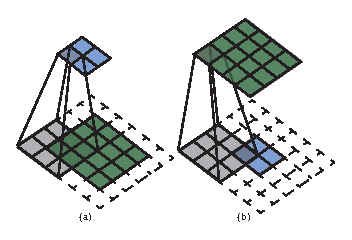
\includegraphics[width=8.5cm]{Figures/Conv_Deconv.eps}
\caption{A diagram of convolution and transposed convolution. The traditional convolution and transposed convolution are shown in the left and right column, respectively.
 The input of convolution is ${4\times4}$, the output is ${2\times2}$ and the kernel is ${3\times3}$. And the transposed convolution is the opposite.}
\label{fig:Deconv}
\end{figure}

If the input and output were to be unrolled into vectors form left to right, top to bottom, the convolution operation can be expressed as:

 \begin{equation}
    \label{Conv_matrix}
    \ y = Wx
\end{equation}

where ${x}$, ${y}$ are flattened vector of input and output. The ${W}$ is a sparse matrix whose non-zero elements are weights of kernels. 
A diagram of conv operation is shown in Fig.~\ref{fig:Deconv}(a). 
For Fig.~\ref{fig:Deconv}(a), ${x}$ is a 16-dimensional vector (the input ${X}$ is a ${4\times4}$ patch), ${y}$ is a 4-dimensional vector and ${W}$ is a matrix of ${4\times16}$.


The output of ${Conv\left\{F_{k}\right\}}$ are upsmapled by a transposed convolution which is written as ${Y = UpSample_n(X)}$, where ${n}$ means ${n}$ times up sampling. The ${n}$ in our network is determined by the size of input $X$ and output $Y$ which is equal to ${max\left\{\lceil Y.weight/X.weight\rceil , \lceil Y.height/X.height\rceil \right\}}$.  Contrary to conv operation, the transposed conv is a process of transforming the features of low dimension to high dimension. It can be written in a inverse form of conv operation:

\begin{equation}
    \label{Conv_matrix}
    \ y = W_1^Tx
\end{equation}

where ${x}$, ${y}$ are flattened vector of input and output. The ${W_1^T}$ is a sparse matrix whose non-zeros elements are weights of deconvolutional kernels. 
Fig.~\ref{fig:Deconv}(b) shows a diagram of transposed conv.
For Fig.~\ref{fig:Deconv}(b), ${x}$ is 4-dimensional vector (the input ${X}$ of transpose conv is a ${2\times2}$ patch), ${y}$ is a 16-dimensional vector and ${W_1^T}$ is a matrix of ${4\times16}$. 

The ${W_1^T}$ of transposed conv layers of different groups are learned separately. It means that the transposed conv layers recovery semantic information from hierarchical feature maps. 
The ${Crop(\left\{X \right\})}$ operation in Part 2 is just a center alignment crop which cuts the superfluous boundary of upsampled feature maps. The output ${\left\{U_k\right\}}$, ${k:\Omega \to\left\{1,\ldots,K\right\}}$ of Part 2 has the same resolution with input ${X}$.

 
\textbf{Part 3} Part 3 is the second fusion stage which aims to fuse the cropped feature maps from Part 2. 
In this part, the fusion operation plays a role of feature weighting.
Using a ${1\times1}$ conv layer, a set of parameters ${w_k}$, ${k:\Omega \to\left\{1,\ldots,K\right\}}$ are learned to combine the hierarchical feature maps.
The expression of the Part 3 is as follows:
\begin{equation}
    \label{fature_selection}
    \ Y= Conv(\left\{U_k\right\})
\end{equation}
where ${Y}$ is output feature map. ${\left\{U_k\right\}}$ is input of Part 3 and output of Part 2.


In order to get a probability map of input ${X}$, the output ${Y}$ of Part 3 is normalized by a sigmoid function:
\begin{equation}
    \label{Sigmoid}
    \ S(x) = \frac{1}{1+e^{-x}}
\end{equation} 
After normalization, A probability map ${P}$ of rooftop is generated, each point in ${P}$ means the probability that pixel belongs to a rooftop. 
If the pixel ${x(i,j)}$ belongs to a roftop, the output ${P(i,j)\approx1}$.

\subsection{Network Training}

The ground truth $G$ in our dataset is labeled by 0 or 1 to indicate whether a pixel belongs to a roof or not. \cxj{only roof? or part of the building including facades?}
When a remote sensing image ${X}$ is inputted into the network, the output is a prediction probability map $P(X;W)$ of roof, where $W$ denotes all the parameters that learned by HF-FCN including first part, Part 2 and 3.
We use the sigmoid cross-entropy loss function to penalize each position on the prediction map formulated as:
\begin{small}
\begin{equation}
     \label{loss}
     \ L(W)\! =\! -\frac{1}{\vert I\vert}\sum_{i=1}^{\vert I \vert}\lbrack{\tilde{g}_i \log{P(X_{i};W)}\!+\!(1\!-\!\tilde{g}_i)\log(1\!-\!P(X_{i};W)}\rbrack
\end{equation}
\end{small}
where $\tilde{g}_i$ is label of $X_{i}$, ${i:\Omega \to\left\{1,\ldots,\vert I\vert\right\}}$, ${\vert I\vert}$ is the number of pixels in the input image ${X}$.

\section{Experiments}
\label{Sec:exp}

To verify the effectiveness of the proposed network, extensive experiments have been conducted on three remote sensing datasets. In this section, the experimental setup is described including details of datasets, training settings of HF-FCN and different criterion for evaluation.


\subsection{Dataset Description}

\paragraph{Massachusetts dataset}
%
Massachusetts dataset consists of 151 aerial images of the Boston area which covers roughly 340 square kilometers.
The resolution of each image is $1500\times 1500$ with the spacial resolution of 1 meter per pixel. And the images are composed of red, green and blue channels.
This dataset is built by Mnih while ground-truth is produced by Saito et al.
The dataset is split into three parts,  a training set of 137 images, a test set of 10 images and validation set of 4 images.
To train the network, we create a set of image tiles for training and validation by sliding a ${256\times256}$ window with 64 stride from right to left, top to bottom. The detailed description is shown in Table \ref{table:dataset-composition}.

\paragraph{Vaihingen dataset}
%
Vaihingen dataset is captured over Vaihingen which is a relatively small village with many detached buildings and small multi story buildings in Germany.
This dataset contains 16 labeled images whose spacial resolution is 9cm per pixel.
It consists of near infra-red, red, green, blue imagery with corresponding normalized digital surface models (nDSMs) and row DSMs. The dataset is divided into training set, validation set, and test set which have 11 images, 2 images, and 3 images respectively. The same crop operations are done as the Massachusetts dataset.

\paragraph{Potsdam dataset}
%
In the Potsdam dataset, there are 24 labeled images whose ground sampling distance is 5cm.
This dataset shows a typical historic city with large building blocks. In order to grasp the global information of the building, the spacial resolution of the original image is reduced from 6000$\times$6000 to 1500$\times$1500.
Each image in this dataset contains 5-channel information: red, green, yellow, DSM and nDSM.
We split the dataset into training, validation and test sets in a proportion of $7:2:1$.



Some measures of data augmentation including data rotation and mirror flipping are made on the three datasets.
Due to the other methods using dataset ${a)}$ do not extend the dataset, so the predict results on the original and extensible dataset $a)$ are both presented to make a fair comparison.
Besides, the data quantity of dataset ${b)}$ and ${c)}$ is not enough to make a adequate training, so we used the extensible dataset as our training set directly.
The components of the datasets are listed in Table~\ref{table:dataset-composition}.
And some sampled patches of dataset ${a)}$, ${b)}$, ${c)}$ are shown in Fig.~\ref{fig:dataset_sample}.
The characteristics and challenges of the three datasets are:
\begin{itemize}
 \item The dataset ${a)}$ has a lot of intensive buildings, which causes great difficulties for the separation of buildings.
 \item There is an obvious shadow occlusion in dataset ${b)}$ which may lead to a wrong segmentation in the part of the shadowed roodtop.
 \item Large intra class differences and small inter class differences are presented in dataset ${c)}$. One building consists of several materials while the roads and buildings are the similar colour. 
\end{itemize}


\begin{figure}
\centering
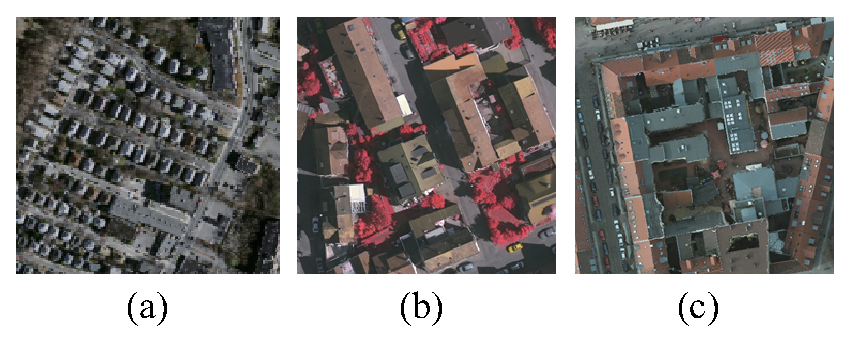
\includegraphics[width=8cm]{Figures/datasets.eps}
\caption{Sample patches on the three datasets  (a) Massachusetts dataset (b) Vaihingen dataset (c) Potsdam dataset}
\label{fig:dataset_sample}
\end{figure}

\begin{table}
 \centering
 \caption{Composition of dataset}
 \label{table:dataset-composition}
 \begin{tabular}{c|ccc}
\hline
& Masschusetts & Vaihingen & Potsdam\\  \hline
Labeled images & 151& 16 &24\\ \hline
GSD & 1m & 9cm & 5cm\\ \hline
Bands & R,G,B & IR,R,G,DSM & IR,R,G,B,DSM\\ \hline
%Training set & \tabincell{c}{1,3,5,7,13,\\17,21,23,26,32,37} &\tabincell{c}{2\_10,3\_10,3\_11,3\_12,\\4\_11,4\_12,5\_10,5\_12,\\6\_8,6\_8,6\_10,6\_11,\\6\_12,7\_7,7\_9,7\_11,7\_12}\\ \hline
Training images &137 & 11 & 17\\ \hline
Training patches&75938 &115088 &85000\\ \hline
Training patch size& 256$\times$256 & 256$\times$256 & 256$\times$256\\ \hline
Validation images & 4 & 3 & 4\\ \hline
validation patches &2500 & 28376 &25000 \\\hline
Validation patch size & 256$\times$256 & 256$\times$256 & 256$\times$256\\ \hline
%Test set & 15,30 &2\_12,6\_7,7\_8 \\ \hline
Test images & 10 & 2 & 3\\ \hline
\end{tabular}
\end {table}



\subsection{Training Settings}
HF-FCN is trained on dataset ${a)}$ firstly owing to large amounts of training data. The pre-trained model of VGG16 Net and ResNet are used to finetune our HF-FCN. We use the stochastic gradient descent algorithm with the learning rate divided by 10 for each 8000 iterations to train our network. The drop-out ratio is set to 0.5 which avoids overfitting. When the HF-FCN converges on the dataset ${a)}$, we transfer it to the other datasets. All experiments in this paper are performed using the deep learning framework Caffe and trained on a single NVIDIA Titan 12GB GPU. Besides, the hyper-parameters are listed in Table~\ref{table:Train-Parameter} \cxj{\Rmnum{3}}.

\begin{table}
\centering
\caption {Parameters for Network Training}
\label{table:Train-Parameter}
\begin{tabular}{c|c|c|c}
\hline
&Massachusetts &Vaihigen &Potsdam\\  \hline
%input size & 256$\times$256 &256$\times$256 \\
mini-batch size & 18& 15 & 15 \\
initial learning rate & $10^{-5}$ & $10^{-6}$ & $10^{-5}$\\
test\_interval&1000 & 1000 &1000\\
%type &SGD &SGD &SGD\\
training iteration & 10000 & 10000& 10000\\
momentum & 0.9 & 0.9 & 0.9\\
clip\_gradients & 16000& 10000 & 10000\\
weight\_decay & 0.02& 0.005 & 0.005\\ \hline
\end{tabular}
\end{table}

\subsection{Evaluation Metrics}
Several evaluation metrics are adopted in our work. For dataset ${a)}$, the most common metrics are correctness (precision) and completeness (recall).
The stantdard ($\rho$=0) and relaxed ($\rho$=3) precision and recall scores are used to evaluate the prediction results. Here the relaxed precision means the predicted pixels are within $\rho$ pixels of a true pixel while the relaxed recall is the true pixels are within $\rho$ pixels of a predicted pixel. Moreover, the time cost is used to measure the efficiency of our HF-FCN. For dataset ${b)}$ and ${c)}$, we use correctness, completeness and F1 score as evaluation metrics.


\begin{equation}
 {completeness} = \frac{TP}{TP+FN},
\end{equation}
\begin{equation}
{correctness} = \frac{TP}{TP+FP},
\end{equation}
\begin{equation}
{F1\_score}= 2\cdot\frac{completeness\cdot correctness}{completeness+correctness}
\end{equation}
%
where TP indicates the true positives, FP implies the false positive, TN means the true negatives and FN refers to the false negatives.

\section{Results and Discussion}
\label{Sec:Res}
In this section, the proposed method using dataset a, b, c are compared to the recent non-deep-learning algorithms, such as Minh-CNN\cite{IEEEexample:mnih2013machine}, Satio-multi\cite{IEEEexample:saito2016multiple} and Context\cite{IEEEexample:audebert2017deep}. Furthermore, it is also compared with some recent deeplearning based approaches, including FCN\cite{IEEEexample:Long_2015_CVPR}, SegNet\cite{IEEEexample:badrinarayanan2017segnet} and etc. Moreover for HF-FCN itself, we expect to investigate the effects of extracted information from different layers on the final prediction. Thus, some variants which combine different up-sampling feature maps from Level 2 are proposed with details shown in Figure 6.\par

\begin{figure}[t]
\begin{center}
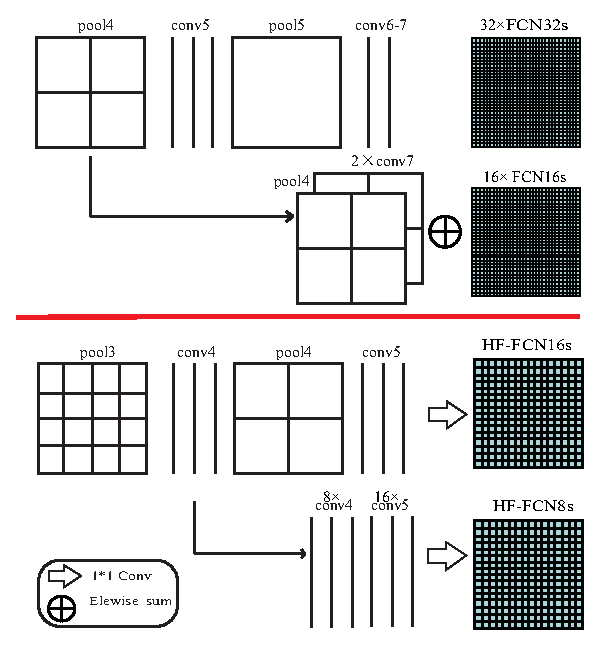
\includegraphics[width=7.8cm]{Figures/vairants.eps}
\caption{HF-FCN variants. The feature maps generated from final group are fused into a coarse result, which is HF-FCN16s. The variant called HF-FCN8s concatenates the feature maps from the last 2 groups with the same fusion operation, and so on.}
\label{6}
\end{center}
\end{figure}

\subsection{Massachusetts dataset}
On the Massachusetts dataset, our method is compared to three state-of-the-art approaches. Table 4 and Figure 7 present the quantitative analysis and precision-recall curves respectively. A standard and relaxed precision and recall are amply to make a comparison. From the reuslt, our method shows obvious superiority in terms of speed and precision. When comparing with Satio\-multi\-MA\&CIS, the standard and relaxed recall are of our method 5.5{\%} and 1.3{\%} higher than it. At the same time, the time coat is reduced from 67.84s to 1.07s and the speed is promoted about 63 times. These significant improvements demonstrate that HF-FCN achieves best performance in effectiveness and efficiency.\par
\setlength{\parindent}{2ex}Meanwhile, extensive comparisons are made between HF-FCN and other mainstream methods in semantic segmentation domain. The visual results are shown in Figure 10. From it, we can see that details and integrity of the building are well preserved by using our method.
\begin{table}
\centering
\caption {Correctness at breakeven of HF-FCN v.s. \cite{IEEEexample:mnih2013machine}\cite{IEEEexample:saito2016multiple}\cite{IEEEexample:alshehhi2017simultaneous} on Massachusetts test set. Cost time is computed in the same computer with a single NVIDIA Titan 12GB GPU}
\begin{tabular}{cccc}
\hline
&Recall ($\rho$ = 3)&Recall ($\rho$ = 0)&Time (s)\\
\hline
Mnih-CNN [9]&0.9271&0.7661&8.70\\
Mnih-CNN+CRF [9]&0.9282&0.7638&26.60\\
Satio-multi-MA [10]&0.9503&0.7873&67.72\\
Satio-multi-MA\&CIS [10]&0.9509&0.7872&67.84\\
Alshehhi-GAP+seg [11]&0.955&{--}&{--} \\
Proposed model (HF-FCN)&0.9643&0.8424&1.07\\ \hline
\end{tabular}
\end{table}

\begin{figure}
\centering
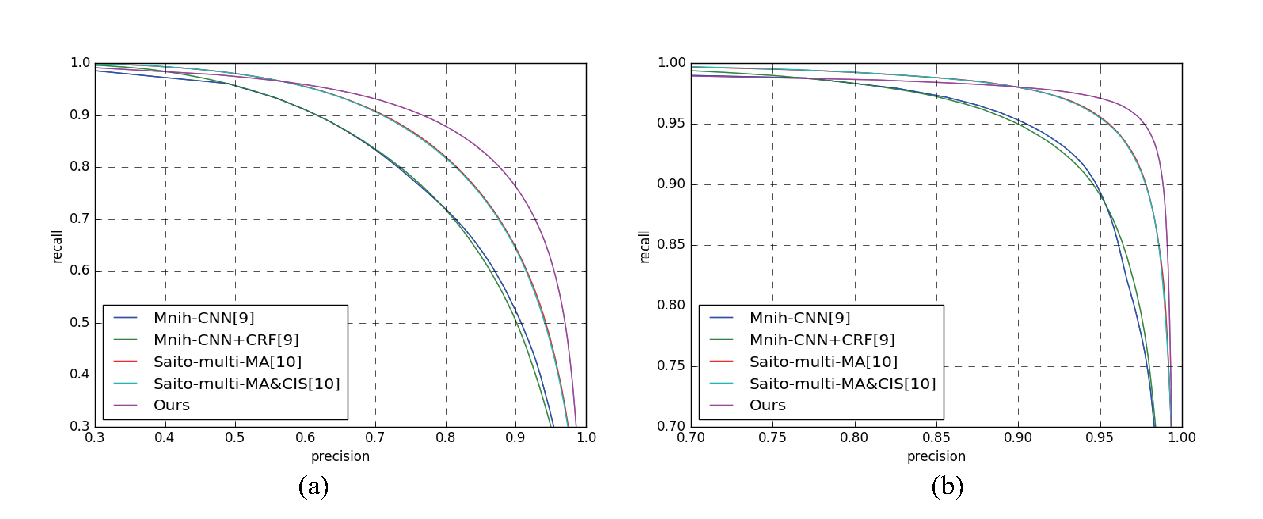
\includegraphics[width=8.7cm]{Figures/HF-FCN_dataset_a.eps}
\caption{The relaxed precision-recall curves from different methods with two slack paramters, (a) $\rho$ = 0; (b) $\rho$ = 3. All curves of our model are located above others.}
\label{7}
\end{figure}
\setlength{\parindent}{2ex}Furthermore, to explore the effects of the feature maps at different scales on the final result, variants of HF-FCN which are counterpart of FCN are designed. Unlike FCN, a fusion operation rather than summing up components in respective locations are leveraged to build our HF-FCN 16s, 8s, 4s. The performance of these variants are shown in Figure 8, Figure 9 and Table \Rmnum{5}. From the disgrams, we get the following conclusions. First, the prediction result obtained from the last layer gets a coarse result, which losts much of location information that mainly encoded in the shallow feature maps. Second, the largest gap presented between HF-FCN16s and HF-FCN8s about 9{\%} in recall rates, it may suggest that the most information supplement to the HF-FCN is got in middle layers. Third, the PR curves of HF-FCN4s and HF-FCN almost coincide. It illustrates the low-level information has little effect on the prediction results. Forth, with the addition of the shallow feature map, the network is more distinct for the segmentation of tiny buildings, which solves the problem of easy adhesion to adjacent buildings. Since, all the Conv layers contained useful hierarchical information that is critical to the final prediction.\par
\setlength{\parindent}{2ex}In the end, we want to prove that fusion operations learn the connections between different features. Connection weights are shown in Figure 11. From the figure, we can see the weights are not the same, which means that fusion operation take effect.
\begin{table}
\centering
\caption {Performance comparison between HF-FCN variants on Massachusetts test set.}
\begin{tabular}{ccc}
\hline
&Recall ($\rho$ = 3)&Recall ($\rho$ = 0)\\
\hline
HF-FCN16s&0.9330&0.7233\\
HF-FCN8s&0.9643&0.8171\\
HF-FCN4s&0.9632&0.8394\\
HF-FCN&0.9643&0.8394\\
\hline
\end{tabular}
\end{table}

\begin{figure}
\centering
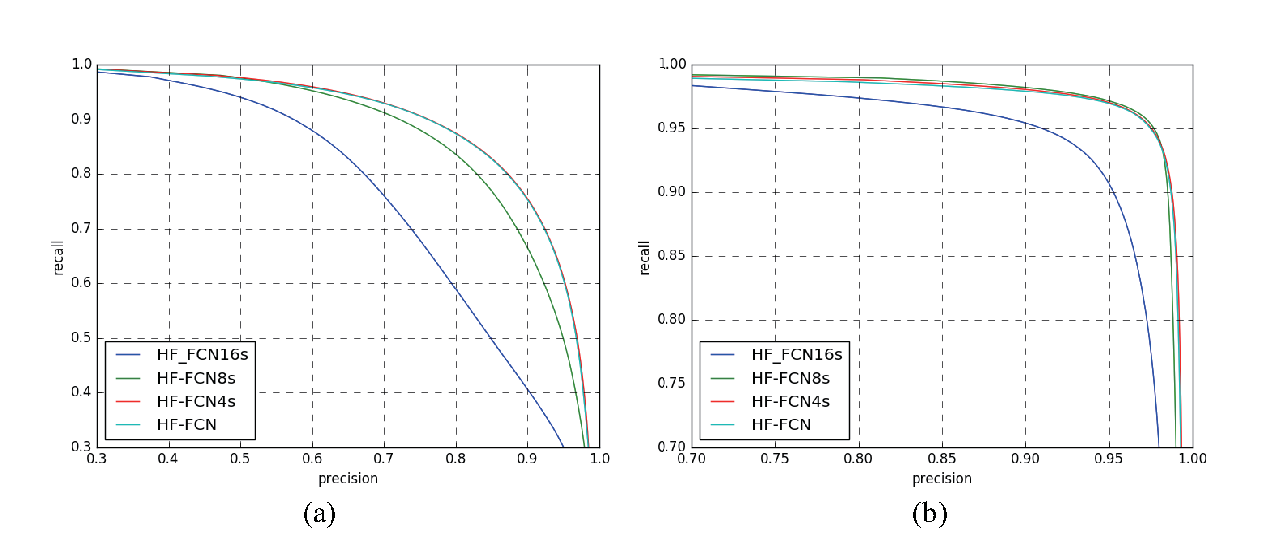
\includegraphics[width=8.7cm]{Figures/HF-FCN-variant-PR.eps}
\caption{The relaxed precision-recall curves from HF-FCN variants with two slack paramters. The biggest gap occurs between HF-FCN16s and HF-FCN8s, which indicates the most additional information coming from middle layers.}
\label{8}
\end{figure}

\begin{figure}
\centering
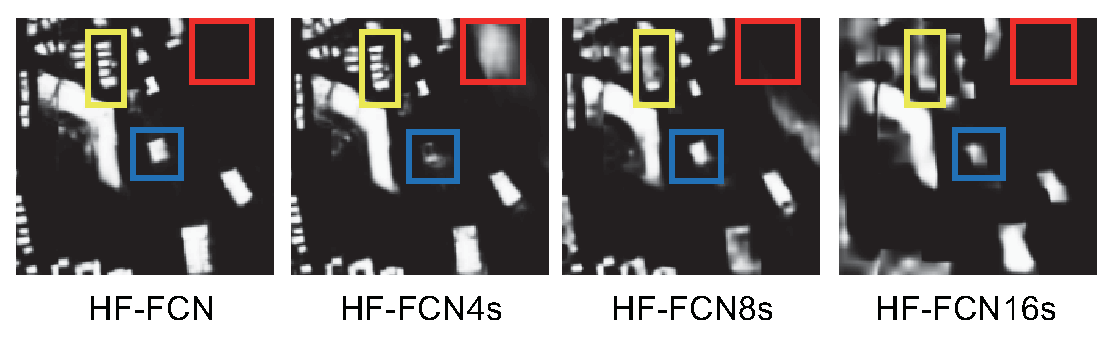
\includegraphics[width=8.7cm]{Figures/HF-FCN_variants_result.eps}
\caption{Prediction results of HF-FCN, HF-FCN4s, HF-FCN8s and HF-FCN16s. The yellow box shows the continuous refinement of the tiny buildings. The red and blue boxes show the mutual promotion and contradiction between different layers.}
\label{9}
\end{figure}

\begin{figure*}
\centering
\includegraphics[width=16.5cm]{Figures/mass_visi_result.eps}
\caption{(a) input images. (b) Results of Mnih-CNN+CRF. (c) Results of Satio\-multi\-MA\&CIS. (d) Results of FCN4s . (e) Results of SegNet. (f) Our results. TP are shown in green, FP are shown in blue and FN are in red.}
\label{10}
\end{figure*}

\begin{figure}
\centering
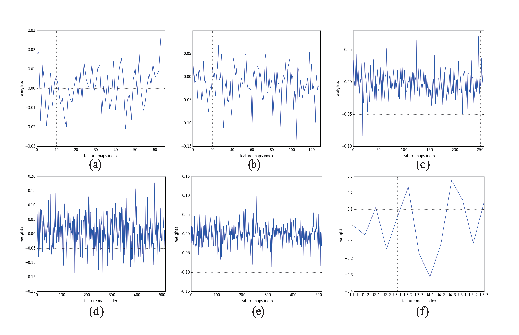
\includegraphics[width=8.4cm, height = 10cm]{Figures/weights.eps}
\caption{(a) is weights learned by F1\_1, (b) is weights learned by F2\_1, (c) is weights learned by F3\_1, (d) is weights learned by F4\_1, (e) is weights learned by F5\_1, (f) is weights learned by Level 2.}
\label{11}
\end{figure}

\subsection{Vaihingen dataset}
On Vaihingen dataset, three experiments are undertaken to explore the effects of different inputs, diverse variants and various methods. We utilize  three kinds of combinations of image channels as inputs. The inputs of the 3 channels are IR, R, G and adding the nDSM as the forth channel. Based on it, DSM is added and made up 5-channel input. We use three standards to make a more comprehensive evaluation. The evaluation results are shown in Table \Rmnum{6}, which illustrates that 3-channel input performed better than the other. Corresponding visual results are shown in Figure 14.\par
\begin{table*}[htbp]
\caption {Performance comparison of the results of different inputs on Vaihigen data set}
\centering
\begin{tabular}{p{1.1cm}<{\centering}|p{1.1cm}<{\centering}|p{1.1cm}<{\centering}|p{1.1cm}<{\centering}|p{1.1cm}<{\centering}|p{1.1cm}<{\centering}|p{1.1cm}<{\centering}|p{1.1cm}<{\centering}|p{1.1cm}<{\centering}|p{1.1cm}<{\centering}|p{1.1cm}<{\centering}}
\hline
&\multirow{2}{*}{Img}&\multicolumn{3}{c}{3\_in: IR, R, G} &\multicolumn{3}{|c|}{4\_in: IR, R, G, nDSM}&\multicolumn{3}{c}{5\_in: IR, R, G, DSM, nDSM}\\
\cline{3-11}
&& Pre &Rec & F1 &Pre &Rec &F1&Pre &Rec &F1\\
\hline
\multirow{3}{*}{Val}&11&0.911&0.906&0.909&0.936&0.900&0.917&0.890&0.900&0.900\\
&28&0.94&0.875&0.906&0.96&0.792&0.868&0.952&0.823&0.883\\
&34&0.965&0.899&0.930&0.987&0.902&0.942&0.972&0.918&0.944\\
&Ave&0.939&0.894&$\bm{0.915}$&0.961&0.865&0.909&0.939&0.880&0.907\\
\hline
\multirow{2}{*}{Test}&15&0.918&0.930&0.924&0.883&0.917&0.9&0.833&0.931&0.88\\
&30&0.921&0.929&0.926&0.931&0.827&0.876&0.875&0.877&0.876\\
&Ave&0.919&0.930&$\bm{0.925}$&0.907&0.872&0.888&0.858&0.900&0.878\\
\hline
\end{tabular}
\end{table*}

\setlength{\parindent}{2ex}The results of diverse variants are shown in Figure 12. From the curves, the performance of HF-FCN exceeds the variants and gets a excellent result. There are some other methods using this dataset. The comparison results are shown in Figure 15. From a visual perspective, our method gets a much more refined roof region. After getting the area of rooftop, the method proposed by \cite{IEEEexample:zhou20112} is used to generate the 3D models. Complete models and details are displayed in Figure 16.

\begin{figure}
\centering
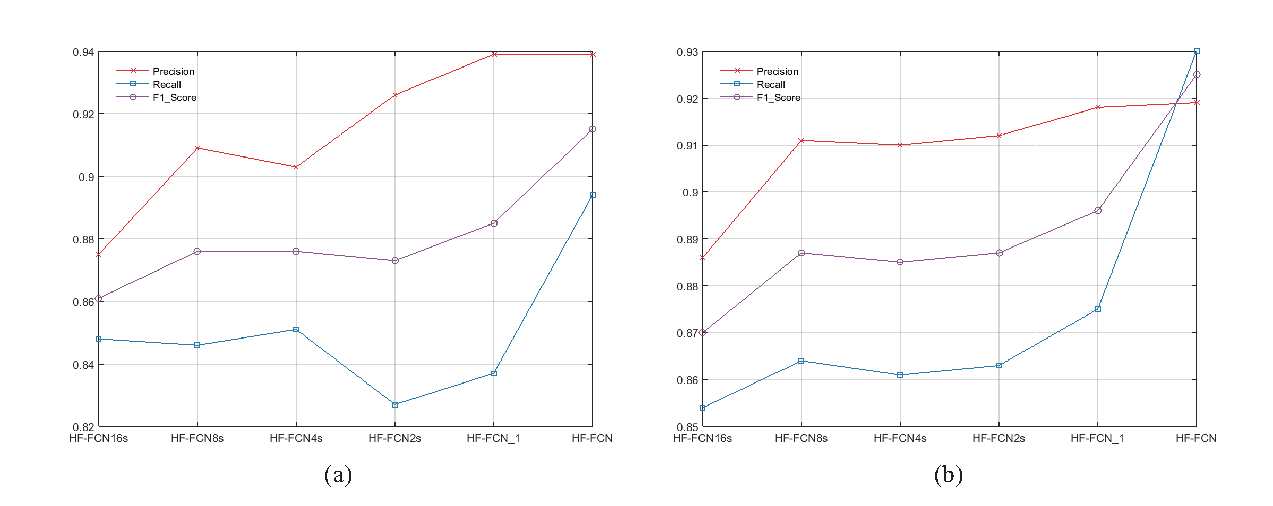
\includegraphics[width=8.7cm]{Figures/vaihingen_variants.eps}
\caption{Results of HF-FCN variants on Vaihingen dataset. (a) (b) shows the precision, recall and F1\_score of validation set and test set of Vaihingen dataset respectively. The HF-FCN\_1 indicates that the last conv layer in Level 2 does not use the previous trained model to initialize. And HF-FCN means that the whole layers use the pre-trained model to initialize.}
\label{12}
\end{figure}

\begin{figure}
\centering
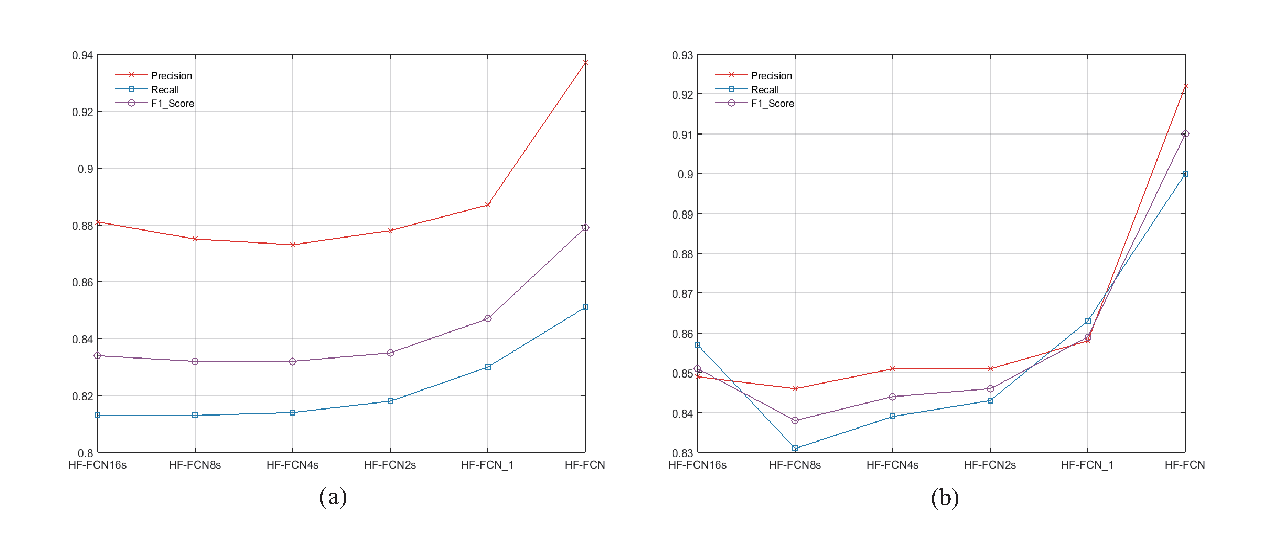
\includegraphics[width=8.7cm]{Figures/Potsdam_variants.eps}
\caption{Results of HF-FCN variants on Potsdam dataset. (a) (b) shows the precision, recall and F1\_score of validation set and test set of Potsdam dataset respectively. The HF-FCN\_1 indicates that the last conv layer in Level 2 does not use the previous trained model to initialize. And HF-FCN means that the whole layers use the pre-trained model to initialize.}
\label{13}
\end{figure}

\begin{figure}
\centering
\includegraphics[width=8.7cm]{Figures/Vaihingen3_4_5in.eps}
\caption{Prediction results on Vaihingen dataset. (a) (b) (c) shows results of the 3-channel input, 4-channel input and 5-channel input of Vaihingen dataset respectively. Here, TP are shown in green, FP are shown in blue and FN are in red.}
\label{14}
\end{figure}

\begin{figure}
\centering
\includegraphics[width=8.7cm]{Figures/Vaihingen_compared_results.eps}
\caption{Results of different methods. (a) is input image, (b)(d)(g) are results of \cite{IEEEexample:audebert2017deep}, (c) is result of \cite{IEEEexample:marmanis2016semantic}, (f) is result of \cite{IEEEexample:unknown}, (g) is our result.}
\label{15}
\end{figure}

\begin{figure}
\centering
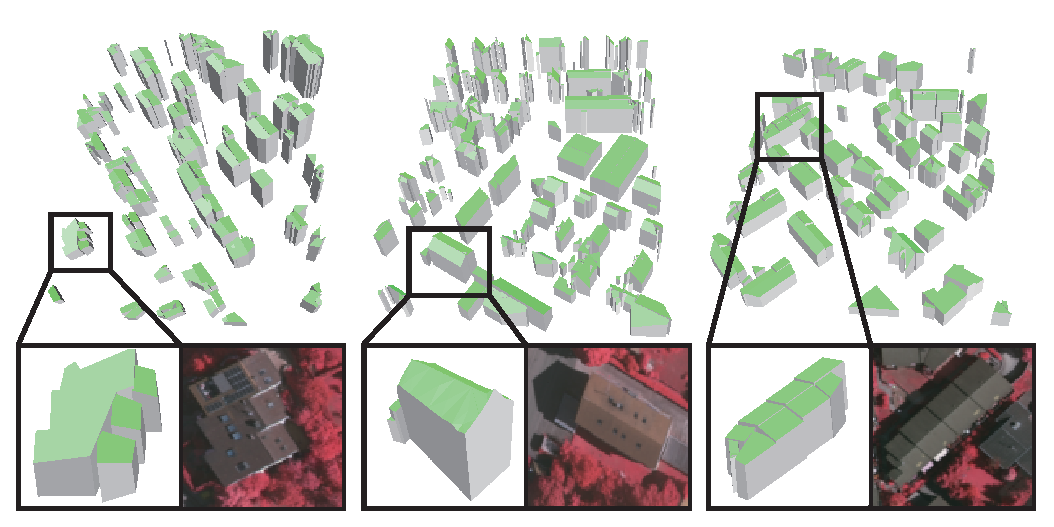
\includegraphics[width=8.7cm]{Figures/Vaihigen_3Dmodelling.eps}
\caption{The 3D modelling of Veihingen dataset. The single building model and its corresponding optical patch were shown together.}
\label{16}
\end{figure}



\subsection{Potsdam dataset}
 The same experiments are implemented on Potsdam dataset. First, We utilize DSM and IR information as extra inputs based on the RGB input. The specific quantitative evaluation and intuitive visual prediction results are shown in Table\Rmnum{7} and Figure 17. In the validation process, the 4-channel input gets better overall performance. Meanwhile, the 5-channel input seems perform better in the course of testing. From the visual results, the 5-channel input network gets lower error detection rate which is shown on the image with small blue areas. And from the 5-channel input to 3-channel input, the F1 score increases from 0.907 to 0.915 on the validation set and increases 0.047 on the test set \par
 \setlength{\parindent}{2ex} As done on Vaihingen dataset, contrast experiments of HF-FCN variants are implemented. The performance curve of HF-FCN variants are shown in Figure 13. We also compare HF-FCN with other methods using the Potsdam dataset. Some qualitative results are shown in Figure 18. HF-FCN got more remarkable segmentation results while edges and details segmentation of other methods do not perform so good. The same way of 3D city modelling is applied to the Potsdam dataset. A few models of scenes are shown in Figure 19.

\begin{table*}[htbp]
    \caption {Performance comparison of the results of different inputs on Potsdam data set}
    \begin{center}
    \begin{tabular}{p{1.1cm}<{\centering}|p{1.1cm}<{\centering}|p{1.1cm}<{\centering}|p{1.1cm}<{\centering}|p{1.1cm}<{\centering}|p{1.1cm}<{\centering}|p{1.1cm}<{\centering}|p{1.1cm}<{\centering}|p{1.1cm}<{\centering}|p{1.1cm}<{\centering}|p{1.1cm}<{\centering}}
     \hline
    &\multirow{2}{*}{Img}&\multicolumn{3}{c}{3\_in:RGB} &\multicolumn{3}{|c|}{4\_in:RGB,IR}&\multicolumn{3}{c}{5\_in:RGB,IR,nDSM}\\
     \cline{3-11}
    && Pre &Rec & F1 &Pre &Rec &F1&Pre &Rec &F1\\
    \hline\hline
    \multirow{4}{*}{Val}&2\_11&0.917&0.950&0.933&0.917&0.978&0.946&0.934&0.976&0.954\\
    &4\_10&0.937&0.945&0.941&0.926&0.943&0.936&0.947&0.946&0.946\\
    &5\_11&0.930&0.972&0.950&0.959&0.975&0.966&0.956&0.977&0.967\\
    &7\_10&0.964&0.536&0.689&0.950&0.590&0.728&0.939&0.554&0.697\\
    \cline{2-11}
    &{Average}&0.937&0.851&0.879&0.937&$\bm{0.872}$&$\bm{0.894}$&$\bm{0.944}$&0.864&0.891\\
    \hline\hline
    \multirow{3}{*}{Test}&2\_12&0.897&0.868&0.882&0.920&0.959&0.939&0.944&0.965&0.955\\
    &6\_7&0.894&0.902&0.898&0.915&0.909&0.912&0.901&0.918&0.909\\
    &7\_8&0.975&0.929&0.951&0.977&0.950&0.957&0.976&0.946&0.960\\
    \cline{2-11}
    &{Average}&0.922&0.900&0.910&0.937&0.935&0.936&$\bm{0.940}$&$\bm{0.943}$&$\bm{0.941}$\\
    \hline\hline
   \end{tabular}
   \end{center}
   \end{table*}

\begin{figure}
\centering
\includegraphics[width=8.7cm]{Figures/Potsdam3_4_5in.eps}
\caption{Prediction results on potsdam dataset. (a) (b) (c) shows results of the 3-channel input, 4-channel input and 5-channel input of Vaihingen dataset respectively. Here, TP are shown in green, FP are shown in blue and FN are in red.}
\label{17}
\end{figure}

\begin{figure}
\centering
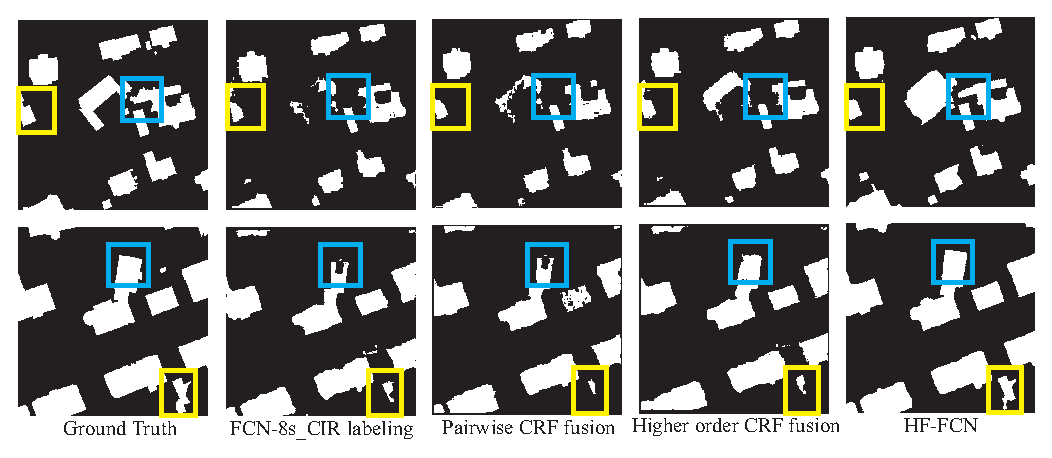
\includegraphics[width=8.7cm]{Figures/Potsdam_compared_results.eps}
\caption{Results of different methods. The second column is the results of using only the FCN with CIR. Pairwise CRF fusion shows the result of fusing FCN-8s\_CIR with LiDAR data in a pairwise CRF. Higher-order CRF are used to generate the results shown in third column. Our results are shown in last colunm.}
\label{18}
\end{figure}

\begin{figure}
\centering
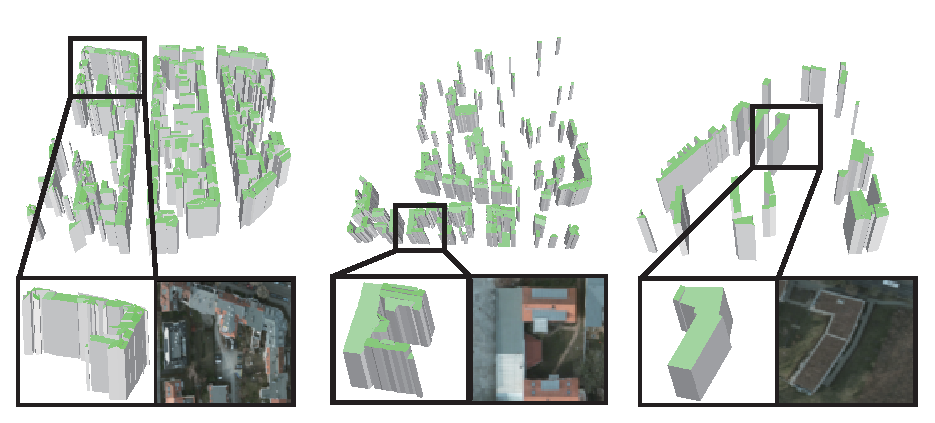
\includegraphics[width=8.7cm]{Figures/potsdam_models.eps}
\caption{The 3D modelling of Potsdam dataset. The single building model and its corresponding optical patch were shown together.}
\label{19}
\end{figure}

\section{Conclusion}
\label{Sec:Con}
 In this paper, we propose a complete system for efficient 3D city modelling from large-scale aerial images via deep learning. A novel CNN architecture, HF-FCN, combines hierarchical semantic layers and multi-scale feature representation to implement final building detection. We design a fusion branch to combine the feature maps stage by stage. And the resulting HF-FCN method shows significant improvements over several previous methods. Distinct from the previous deeplearning based methods, we utilize the multi-scale inherent information within the CNN and get fine detail detection results. Unlike existing 3D  reconstruction methods, our proposed approach relies on the HF-FCN to efficiently extract the area of buildings to build the 3D models of the geospatial objects. Finally, our study suggests that even with the powerful semantic expressive ability of CNNs and their good robustness to scale, it is still critical to address multi-scale problems utilizing hierarchical feature maps encoded in CNNs.


\bibliographystyle{IEEEtran}
\bibliography{IEEEexample}
\end{document}


